\clearpage

\section{Carrier Phase Compensation}

\begin{tcolorbox}	
	\begin{tabular}{p{2.75cm} p{0.2cm} p{10.5cm}} 	
		\textbf{Header File}   &:& carrier\_phase\_estimation$\_*$.h \\
		\textbf{Source File}   &:& carrier\_phase\_estimation$\_*$.cpp \\
        \textbf{Version}       &:& 20180423 (Celestino Martins) \\
	\end{tabular}
\end{tcolorbox}

This block performs the laser phase noise compensation using either Viterbi-Viterbi (VV) algorithm or blind phase search algorithm (BPS). For both cases, it receives one input complex signal and outputs one complex signal.

\subsection*{Input Parameters For VV Algorithms}

\begin{table}[h]
	\centering
	\begin{tabular}{|c|c|c|c|cccc}
		\cline{1-4}
		\textbf{Parameter} & \textbf{Type} & \textbf{Values} &   \textbf{Default}& \\ \cline{1-4}
		nTaps              & int & any & $25$ \\ \cline{1-4}
        methodType         & string & VV & VV \\ \cline{1-4}
		mQAM                  & int & any & $4$ \\ \cline{1-4}		
	\end{tabular}
	\caption{CPE input parameters}
	\label{table:cpe_in_par_vv}
\end{table}


\subsection*{Input Parameters For BPS Algorithms}

\begin{table}[h]
	\centering
	\begin{tabular}{|c|c|c|c|cccc}
		\cline{1-4}
		\textbf{Parameter} & \textbf{Type} & \textbf{Values} &   \textbf{Default}& \\ \cline{1-4}
		nTaps              & int & any & $25$ \\ \cline{1-4}
        NtestPhase         & int & any & $32$ \\ \cline{1-4}
        methodType         & string & BPS & VV \\ \cline{1-4}
		mQAM                  & int & any & $4$ \\ \cline{1-4}	
	\end{tabular}
	\caption{CPE input parameters}
	\label{table:cpe_in_par_bps}
\end{table}

\subsection*{Methods}

CarrierPhaseCompensation() {};
\bigbreak
CarrierPhaseCompensation(vector$<$Signal *$>$ \&InputSig, vector$<$Signal *$>$ \&OutputSig) :Block(InputSig, OutputSig)\{\};
\bigbreak
void initialize(void);
\bigbreak
bool runBlock(void);
\bigbreak
void setnTaps(int ntaps) { nTaps = ntaps; }
\bigbreak
double getnTaps() { return nTaps; }
\bigbreak
void setmQAM(int mQAMs) { mQAM = mQAMs; }
\bigbreak
double getmQAM() { return mQAM; }
\bigbreak
void setTestPhase(int nTphase) { nTestPhase = nTphase; }
\bigbreak
double getTestPhase() { return nTestPhase; }
\bigbreak
void setmethodType(string mType) { methodType = mType; }
\bigbreak
string getmethodType() { return methodType; }
\bigbreak
void setBPStype(string tBPS) { BPStype = tBPS; }
\bigbreak
string getBPStype() { return BPStype; }

\subsection*{Functional description}

This block can perform the carrier phase noise compensation originated by the laser source and local oscillator in coherent optical communication systems. For the sake of simplicity, in this simulation we have restricted all the phase noise at the transmitter side, in this case generated by the laser source, which is then compensated at the receiver side using DSP algorithms.
In this simulation, the carrier phase noise compensation can be performed by applying either the well known Viterbi-Viterbi (VV) algorithm or blind phase search algorithm (BPS), by configuring the parameter $methodType$. The parameter $methodType$ is defined as a string type and it can be configured as: i) When the parameter $methodType$ is $\textit{VV}$ it is applied the VV algorithm; When the parameter $methodType$ is $\textit{BPS}$ it is applied the BPS algorithm.

\subsubsection{Viterbi-Viterbi Algorithm}
\begin{figure}[h!]
    \centering
    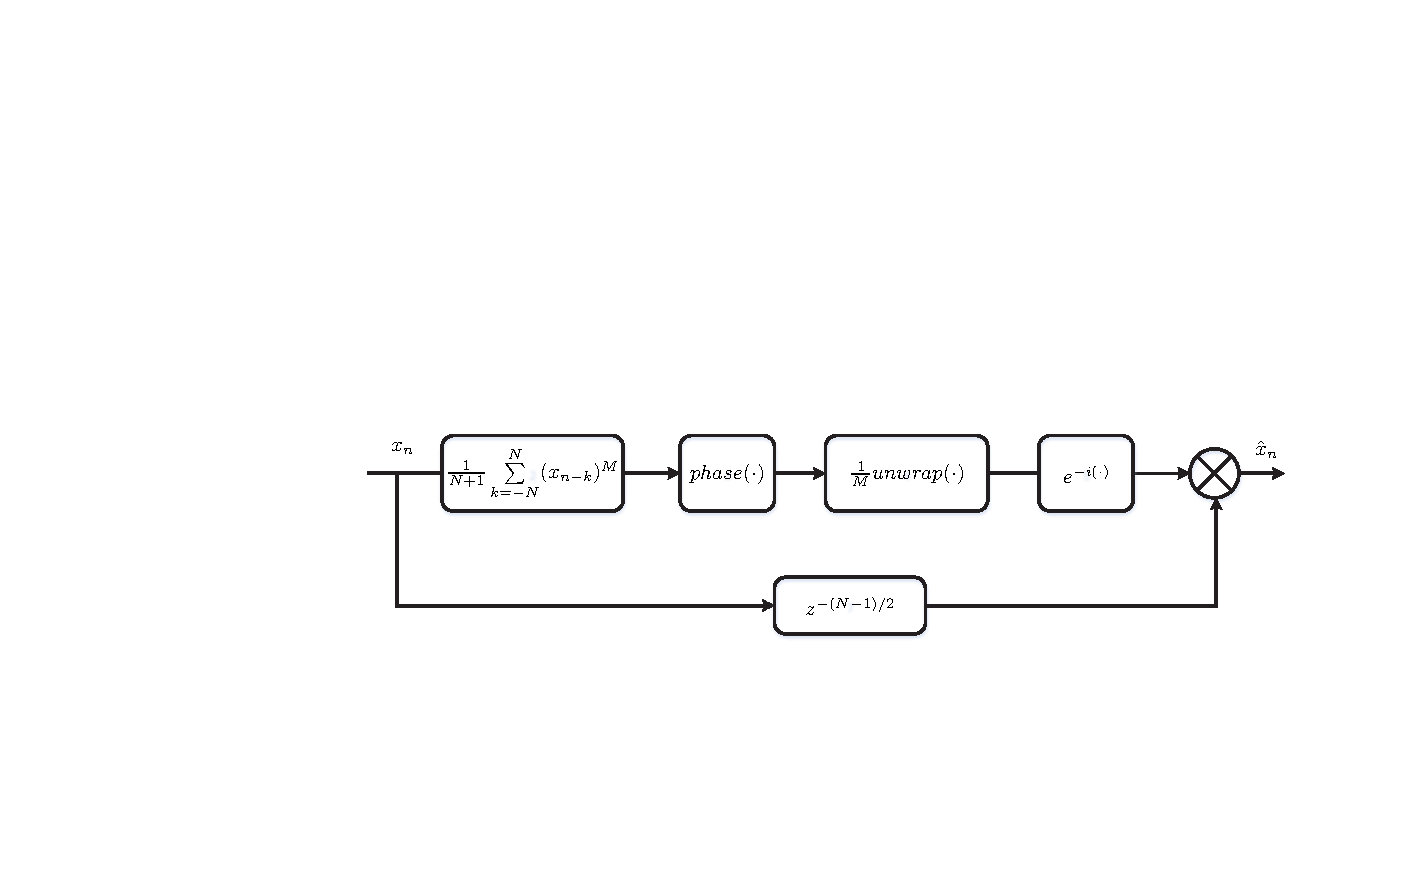
\includegraphics[width=\textwidth]{./lib/carrier_phase_estimation/figures/VV_phaseEstimation.pdf}
    \caption{Block diagram of Viterbi-Viterbi algorithm for carrier phase recovery.}
    \label{fig_VVdiagram}
\end{figure}
VV algorithm is a n-th power feed-forward approach employed for uniform angular distribution characteristic of m-PSK constellations, where the information of the modulated phase is removed by employing the n-th power operation on the received symbols. The algorithm implementation diagram is shown in Figure~\ref{fig_VVdiagram}, starting with M-th power operation on the received symbols. In order to minimize the impact of additive noise in the estimation process, a sum of $2N+1$ symbols is considered, which is then divided by M. The resulting estimated phase noise is then submitted to a phase unwrap function in order to avoid the occurrence of cycle slip. The final phase noise estimator is then used to compensate for the phase noise of the original symbol in the middle of the symbols block.

\subsubsection{Blind Phase Search Algorithm}
\begin{figure}[h!]
    \centering
    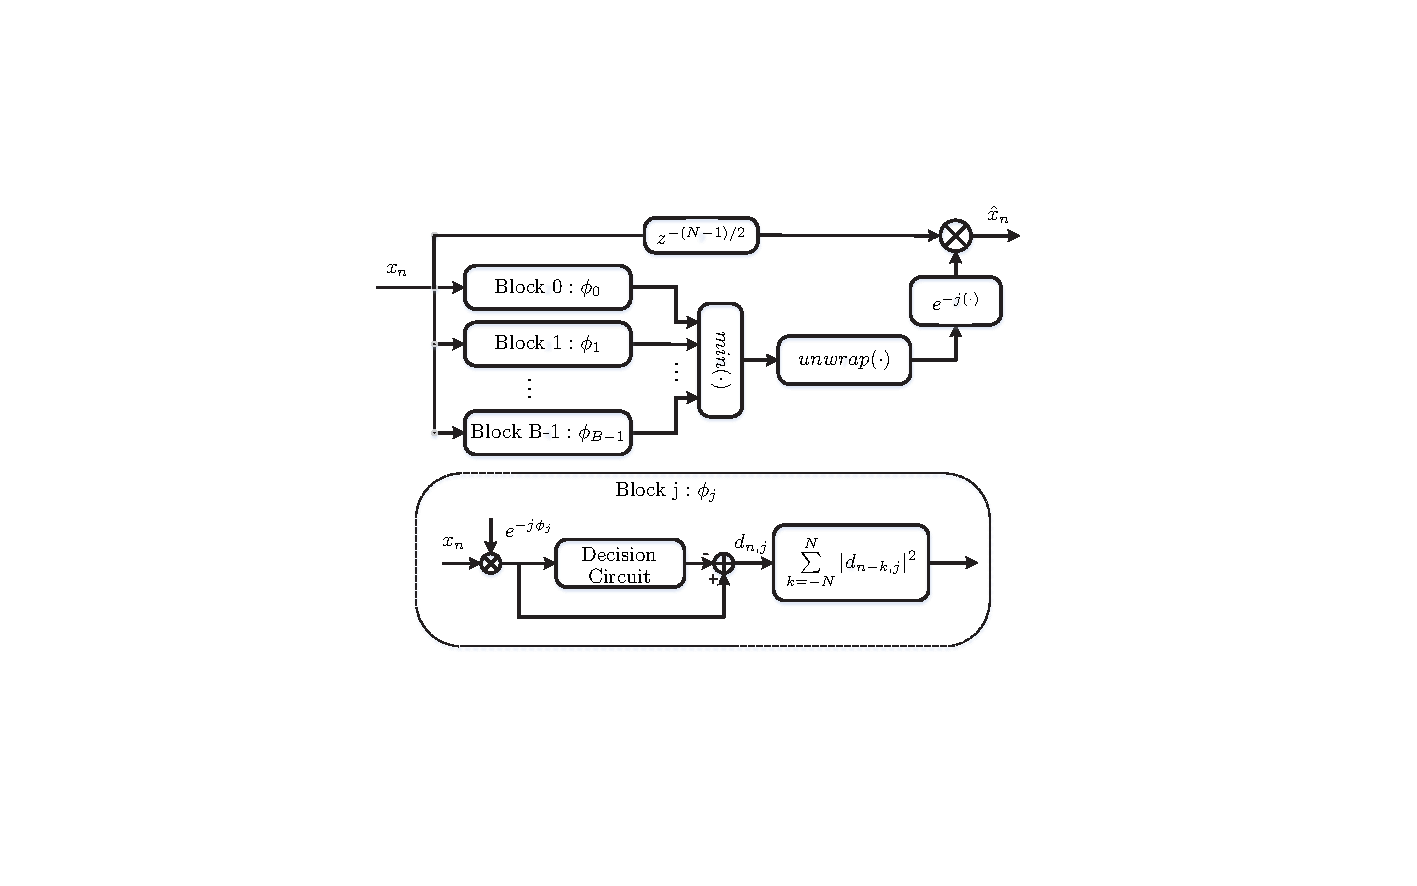
\includegraphics[width=12cm]{./lib/carrier_phase_estimation/figures/bps_diagram.pdf}
    \caption{Block diagram of blind phase search algorithm for carrier phase recovery.}
    \label{fig_BPSdiagram}
\end{figure}
An alternative to the VV phase noise estimator is the so-called BPS algorithm, in which the operation principle is shown in the Figure~\ref{fig_BPSdiagram}. Firstly, a block of $2N+1$ consecutive received symbols is rotated by a number of $B$ uniformly distributed test phases defined as,
\begin{equation}
    	\phi_{b} = \frac{b}{B}\frac{\pi}{2}, b \in\{0,1,...,B-1\}.
    \label{eq_phaseNoise}
\end{equation}
Then, the rotated blocks symbols are fed into decision circuit, where the square distance to the closest constellation points in the original constellation is calculated for each block. Each resulting square distances block is summed up to minimize the noise distortion. After average filtering, the test phase providing the minimum sum of distances is considered to be the phase noise estimator for the symbol in the middle of the block. The estimated phase noise is then unwrapped to reduce cycle slip occurrence, which is then used employed for the compensation for the phase noise of the original symbols.

\pagebreak
\subsection*{Input Signals}

\subparagraph*{Number:} 1

\subsection*{Output Signals}

\subparagraph*{Number:} 1

\subparagraph*{Type:} Electrical complex signal

\subsection*{Examples}

\subsection*{Sugestions for future improvement}


